\subsection{Widening Operation for \tia}

\begin{figure}[tp]
    \hfill
    \begin{subfigure}[b]{.3\textwidth}
        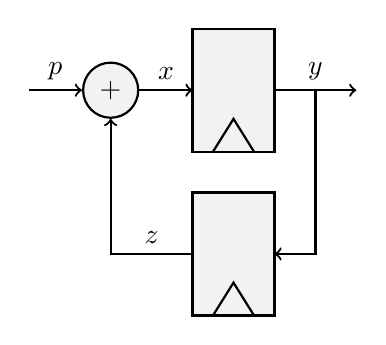
\begin{tikzpicture}[scale=0.52,thick]
    % adder
    \node[circle,draw,minimum size=.7cm,fill=gray!10] (a) at (0,0) {\textred{$+$}};
    \draw[->] (-2,0) --node[above]{\textpurple{$p$}} (a);
    \draw[->] (a) --node[above]{$x$} (2,0);
    % register1
    \draw[fill=gray!10] (2,-1.5) rectangle (4,1.5);
    \draw (2.5,-1.5) -- (3,-0.7) -- (3.5,-1.5);
    \draw[->] (4,0) --node[above]{$y$} (6,0);
    % register2
    \draw[fill=gray!10] (2,-5.5) rectangle (4,-2.5);
    \draw (2.5,-5.5) -- (3,-4.7) -- (3.5,-5.5);
    \draw[->] (5,0) -- (5,-4) -- (4,-4);
    \draw[->] (2,-4) --node[above]{$z$} (0,-4) -- (a);
\end{tikzpicture}

        \caption{The circuit under analysis.}
    \end{subfigure}
    \hfill
    \begin{subfigure}[b]{.6\textwidth}
        \centering
        \[
        \left\{ x = \textpurple{p} + z,\ y \Leftarrow x,\ z \Leftarrow y\right\}
        \]
        \caption{Formal representation of this circuit.}
        \vspace{1ex}
        \begin{tikzpicture}[scale=1,thick]
    \node (p) at (0, 0) {$\textpurple{p}$};
    \node[fill=gray!10] at (0, 0.75) {$\{o_p^0\}$};

    \node (x) at (2, 0) {$x$};
    \node[fill=gray!10] at (2, 0.75) {$\{o_p^{2i}\mid i \in \nats\}$};

    \node (y) at (3, -1) {$y$};
    \node[fill=gray!10,right=3pt of y] {$\{o_p^{2i + 1}\mid i \in \nats\}$};

    \node (z) at (1, -1) {$z$};
    \node[fill=gray!10,left=3pt of z] {$\{o_p^{2i + 2}\mid i \in \nats\}$};

    \draw [->] (p) -- (x);
    \draw [->] (x) --node[above right]{$1$} (y);
    \draw [->] (y) --node[below]{$1$} (z);
    \draw [->] (z) -- (x);
\end{tikzpicture}

        \caption{\tia's result for this circuit.}
    \end{subfigure}
    \hfill
    \caption{An example of temporal influence analysis (\tia) with infinite temporal influence objects.}\label{fig:inf}
\end{figure}

A practical challenge in implementing \tia is that the set of temporal influence objects associated with a circuit location can be infinite.
Figure~\ref{fig:inf} illustrates such an example, where a feedback loop can propagate an input port's influence across arbitrarily many clock cycles, resulting in infinitely many temporal influence objects.
Consequently, a direct worklist algorithm that computes the fixed point of Definition~\ref{def:tia} may fail to terminate.
To address this issue, we introduce a widening operation $\widening : \powerset(\objects) \to \powerset(\objects)$ for \tia, given in Algorithm~\ref{alg:widening}.
The widening operation replaces larger sets of temporal influence objects with arithmetic progressions, which can be represented compactly using only the initial term and common difference.

Consider the successive analysis results for $\absT(y)$ in the \tia example of Figure~\ref{fig:inf}:
\[
\emptyset \xrightarrow{ \tia } \{o_p^1\} \xrightarrow{ \tia } \{o_p^1, o_p^3\} \xrightarrow{ \tia } \{o_p^1, o_p^3, o_p^5\} \xrightarrow{ \tia } \{o_p^1, o_p^3, o_p^5, o_p^7\} \xrightarrow{ \tia } \dots
\]
This sequence does not reach a finite fixed point because the set of temporal influence objects grows indefinitely.
Now consider a widening threshold of $N=3$ in
Algorithm~\ref{alg:widening}, and apply $\widening$ whenever $\absT$ changes.
After the third temporal influence object is discovered, widening replaces the finite set with the corresponding arithmetic progression:
\[
\emptyset \to \{o_p^1\} \xrightarrow{ \tia } \{o_p^1, o_p^3\} \xrightarrow{ \tia } \{o_p^1, o_p^3, o_p^5\} \xrightarrow{ \widening } \{o_p^{1+2i}\mid i \in \nats\} \xrightarrow{ \tia } \{o_p^{1+2i}\mid i \in \nats\}\ \text{(fixed point)}
\]
Thus, widening allows the analysis to represent the infinite set of temporal influence objects compactly and reach a fixed point after a finite number of iterations.

\begin{algorithm}[tp]
    \caption{Widening Operation for \tia}\label{alg:widening}
    \begin{algorithmic}[1]
        \Require a set of temporal influence objects $O$
        \Ensure a widened set of temporal influence objects $O'$ such that $O \subseteq O'$
        \State Let $N > 1$ be a threshold for triggering widening.
        \Procedure{TiaWidening}{$O$}:
        \State $O' := \emptyset$
        \ForAll{$p \in \ports$}
        \label{line:port}
        \State $O_p := \{o_p^i \in O\}$ \label{line:origin}
        \Comment{Gets the influence objects of port $p$.}
        \If{$|O_p| \ge N$} \label{line:threshold}
        \Comment{Widens $O_p$ to an arithmetic progression.}
        \State $a := \min\{i \mid o_p^i \in O_p\}$ \label{line:init}
        \Comment{Initial term.}
        \State $d := \gcd\{ |i - j | \mid o_p^i, o_p^j \in O_p\}$ \label{line:diff}
        \Comment{Common difference.}
        \State $O_p := \{o_p^{a + di} | i\in \nats\}$ \label{line:widened}
        \Comment{Represented compactly by $a$ and $d$.}
        \EndIf
        \State $O' := O' \cup O_p$
        \EndFor
        \State \Return $O'$
        \EndProcedure
    \end{algorithmic}
\end{algorithm}

\paragraph{Soundness and Convergence Property of \widening}

Next, we prove the soundness and convergence properties of this widening operation.

\begin{theorem}[Soundness of \widening]\label{theo:widening-soundness}
    The widening operation $\widening : \powerset(\objects) \to \powerset(\objects)$ defined by Algorithm~\ref{alg:widening} is sound, i.e.,
    \[
    \forall O \in \powerset(\objects).\ O \subseteq \widening(O).
    \]
\end{theorem}
\begin{proof}
    It suffices to show that, for every $p \in \ports$, the resulting set $O_p$ at Line~\ref{line:widened} is a superset of the original set $O_p$ at Line~\ref{line:origin} when widening is triggered.
    Let $O_p'$ denote the widened set at Line~\ref{line:widened}.
    Consider any $o_p^k \in O_p$.
    By Line~\ref{line:init}, $a = \min\{i \mid o_p^i \in O_p\}$, so $k-a \ge 0$.
    Moreover, by Line~\ref{line:diff}, $d = \gcd\{ |i-j| \mid o_p^i,o_p^j \in O_p\}$.
    Thus, $d$ divides $|k-a| = k-a$, and hence there exists some
    $i \in \nats$ such that $k-a = di$.
    Therefore, $k = a + di$, which implies $o_p^k \in O_p'
    = \{o_p^{a+di} \mid i \in \nats\}$.
    Hence $O_p \subseteq O_p'$.
\end{proof}

By Theorem~\ref{theo:widening-soundness}, applying $\widening : \powerset(\objects) \to \powerset(\objects)$ after each $\tia$ update of $\absT(l) \in \powerset(\objects)$ preserves soundness for every location $l$, since widening only adds temporal influence objects to $\absT(l)$ and therefore cannot remove any information established by $\tia$.

\begin{theorem}[Convergence of \widening]\label{theo:widening-convergence}
    For an arbitrary sequence of temporal influence object sets $O_0,O_1,O_2,\dots \subseteq \objects$ such that $O_0$ is finite and
    \[
    \forall i \in \nats.\ O_{i+1} = \widening(O_i \cup \{o_{p_i}^{k_i}\})
    \]
    for some $p_i \in \ports$ and $k_i \in \nats$, the sequence eventually reaches a fixed point (i.e., converges):
    \[
    \exists n \in \nats.\ O_n = O_{n+1} = O_{n+2} = \cdots.
    \]
\end{theorem}
\begin{proof}
    Without loss of generality, we first make two assumptions that simplify the proof:
    \begin{enumerate}[leftmargin=*]
        \item
        It suffices to consider the evolution of the temporal influence objects associated with a single input port $p$, since $\widening$ processes the objects associated with each input port independently by Line~\ref{line:port} of Algorithm~\ref{alg:widening}.
        Thus, we assume that every object in $O_i$ has the form $o_p^j$.
        \item
        We assume that $|O_0| \geq N$.
        If the sequence reaches a fixed point before the widening threshold is reached, the theorem already holds.
        Otherwise, since each step adds at most one new temporal influence object, the sequence reaches the threshold after finitely many steps.
        We can therefore take the first set at which widening is triggered as the new $O_0$.
    \end{enumerate}
    From this point onward, every $O_i$ ($i \ge 1$) has the form
    \[
    O_i = \{o_p^{a + d j} \mid j \in \nats\}
    \]
    for some $a,d \in \nats$.
    Now define a potential function $\varphi : \{O_i \mid i \ge 1\} \to \nats$ as
    \[
    \varphi\left(\{o_p^{a + dj} \mid j \in \nats\}\right) = a + d.
    \]
    Since $\nats$ is well ordered and therefore admits no infinite strictly decreasing sequence, it suffices to show that
    \begin{equation}\label{eq:potential}
        \forall i \ge 1.\ O_{i+1} \ne O_{i} \Rightarrow \varphi(O_{i+1}) < \varphi(O_{i}).
    \end{equation}
    This ensures that the sequence can change only finitely many times, and therefore must eventually reach a fixed point.

    \paragraph{Proof of Equation~\eqref{eq:potential}}
    Consider any $i \geq 1$ and suppose
    \[
    O_i = \{o_p^{a + d j} \mid j \in \nats\}
    \]
    and
    \[
    O_{i+1} = \widening(O_i \cup \{o_p^k\}) = \{o_p^{a'+d'j}\mid j\in\nats\}
    \]
    for some $a,d, k, a', d' \in \nats$.
    Since $O_{i+1}\neq O_i$, we must have $o_p^k\notin O_i$.
    We consider two cases:

    \noindent
    (1) Case $k < a$:
    Since $k$ is the new minimum, we have $a' = k < a$ by Line~\ref{line:init} of Algorithm~\ref{alg:widening}.
    Moreover, all differences between elements of $O_i$ are multiples of $d$, so the new common difference is $d' = \gcd(a - k, d)$ by Line~\ref{line:diff} of Algorithm~\ref{alg:widening}.
    Therefore,
    \[
    \varphi(O_{i+1}) = a' + d' < a + d' = a + \gcd(a - k, d) \le a + d = \varphi(O_i).
    \]

    \noindent
    (2) Case $k > a$:
    The new minimum remains $a$, so $a' = a$ by Line~\ref{line:init} of Algorithm~\ref{alg:widening}.
    Moreover, the new common difference $d' = \gcd(k - a, d)$ by Line~\ref{line:diff} of Algorithm~\ref{alg:widening}.
    Since $o_p^k \notin O_i$, $k-a$ is not divisible by $d$.
    Thus, $\gcd(k - a, d) < d$ and consequently
    \[
    \varphi(O_{i+1}) = a + d' = a + \gcd(a - k, d) < a + d = \varphi(O_i).
    \]
    Therefore, in both cases, $O_{i+1} \neq O_i \Rightarrow
    \varphi(O_{i+1}) < \varphi(O_i)$, which proves Equation~\eqref{eq:potential}.
\end{proof}

By Theorem~\ref{theo:widening-convergence}, applying $\widening : \powerset(\objects) \to \powerset(\objects)$ after each $\tia$ update of $\absT(l) \in \powerset(\objects)$ ensures that the evolution of $\absT(l)$ eventually reaches a fixed point for every location $l$.
Consequently, the widened version of $\tia$ eventually converges.